% Technische Formelsammlung by Emu

% Dokumenteinstellungen
\documentclass[10pt,a4paper]{scrartcl}
\usepackage[a4paper]{geometry}
\usepackage[utf8x]{inputenc}
\usepackage{amsmath}
\usepackage{amssymb}
\usepackage{esint}
\usepackage{color}
\usepackage{graphicx}
\usepackage{multicol}
\usepackage{multirow}
\usepackage{booktabs}
\usepackage{watermark}
\usepackage{array}
\usepackage{undertilde}
\usepackage{pbox}			%Intelligent parbox: \pbox{maximum width}{blabalbalb \\ blabal}


% Dokumentbeschreibung
\title{Algorithmen und Datenstrukturen Zusammenfassung}
\author{Emanuel Regnath}
\watermark{ \centering \put(0,-500){ \includegraphics {./img/watermark.pdf} } }






% Eigene Befehle
\newcommand{\todayV}{\the\day.\the\month.\the\year}                          %%D.M.YYYY
\newcommand{\iset}[2]{\ensuremath{\bigl\{ \bigl. #1 \, \bigr| \, #2 \bigr\}}}	%intensional set
\newcommand{\eset}[1]{\ensuremath{\bigl\{#1\bigr\}}}							%extensional set
\newcommand{\norm}[1]{\ensuremath{\|#1\|}}										%Norm
\newcommand{\gk}[1]{\ensuremath{\left\lfloor#1\right\rfloor}} 					%Gaußklammer
\newcommand{\sprod}[2]{\ensuremath{\left\langle #1, #2 \right\rangle }}			%Skalarprodukt
\newcommand{\abs}[1]{\ensuremath{\left\vert#1\right\vert}} 						%Betrag
\newcommand{\mat}[1]{\ensuremath{\begin{bmatrix} #1 \end{bmatrix}}}				%Matrix
\newcommand{\vect}[1]{\ensuremath{\begin{pmatrix} #1 \end{pmatrix}}}			%Vektor
\newcommand{\mvect}[1]{\ensuremath{\left. \begin{matrix} #1 \end{matrix}  \right]}} %Matrixvektor
\newcommand{\ma}[1]{\ensuremath{\utilde{\bs {#1}}}}

% Abkürzungen
\newcommand{\ul}[1]{\ensuremath{\underline{#1}}}								%Untersteichen
\newcommand{\ol}[1]{\ensuremath{\overline{#1}}}									%Überstreichen
\newcommand{\Ra}[0]{\ensuremath{\Rightarrow}}									%Rightarrow
\newcommand{\ra}[0]{\ensuremath{\rightarrow}} 									%Rightarrow
\newcommand{\n}[0]{\ensuremath{\overline}}										%NOT
\newcommand{\bs}[1]{\ensuremath{\boldsymbol{#1}}}								%Fett und kursiv im mathmode
\newcommand{\diff}{\ensuremath{\ \mathrm d}}									%delta
\newcommand{\grad}{\ensuremath{\mathrm{grad}\ }}								%Gradient
\renewcommand{\div}{\ensuremath{\mathrm{div}\ }}								%Divergenz
\newcommand{\rot}{\ensuremath{\mathrm{rot}\ }}									%Rotation
\newcommand{\Sp}{\ensuremath{\mathrm{Sp}\ }}									%Spur
	% Für Mengen
	\newcommand{\N}{\ensuremath{\mathbb N}}
	\newcommand{\R}{\ensuremath{\mathbb R}}
	\newcommand{\C}{\ensuremath{\mathbb C}}



% Dokumentbeginn
\begin{document}

% Titel
\maketitle


Ich übernehme keine Gewähr für Vollständigkeit oder Korrektheit!\\
Fehler bitte an emanuel.regnath@tum.de senden! Hompage: www.emareg.de\\



% -------------------------------------------
% | 		Algorithmen und Datenstrukturen	|
% ~~~~~~~~~~~~~~~~~~~~~~~~~~~~~~~~~~~~~~~~~~~
% =============================================================================================================================
\section{Allgemeines}
% ==========================================================================================================

\subsection{Mengenalgebra}
Potenzmenge: Die Menge aller Teilmengen. $\mathcal P(A) = \iset{U}{U \subseteq A}$\\
Karthesisches Produkt: $A \times B = \iset{(a,b)}{a \in A \land b \in B}$\\
Zwei Mengen $A$ und $B$ heißen disjunkt, wenn $A \cap B = \emptyset$\\

\subsubsection{Relationen}
Eine zweistellige Relation $R$ zwischen zwei Mengen $A$ und $B$ ist eine Teilmenge von $A \times B$\\
Eigenschaften von $R \subseteq A \times B$:
\begin{description}
	\item[reflexiv:] $\forall a \in A: (a,a)\in R$	\qquad $aRa$ (ist wahr) 
	\item[symmetrisch:] $\forall a,b \in A:(a,b) \in R \Rightarrow (b,a) \in R$ \qquad $aRb \Leftrightarrow bRa$
	\item[antisymmetrisch:] $\forall a,b \in A:(a,b) \in R \land (b,a) \in R \Rightarrow a=b$ \qquad $aRb \ \land \ bRa \Rightarrow a=b$
	\item[transitiv:] $\forall a,b, \in A:(a,b) \in R\land (b,c) \in R \Rightarrow (a,c) \in R$ \qquad $aRb \ \land \ bRc \Rightarrow aRc$
\end{description}

$R$ heißt partielle Ordnung, falls $R$ reflexiv, antisymmetrisch und transitiv ist.\\
$R$ heißt Äquivalenzrelation, falls $R$ reflexiv, symmetrisch und transitiv ist.\\
Eine partielle Ordnung hießt totale Ordnung, falls alle Elemente miteinander vergleichbar sind.\\


\subsection{Abbildung}
Eine Abbildung ist eine Relation $R \subseteq A \times B$: \\
\boxed{ \forall a \in A: | \iset{b \in B}{(a,b)\in R}| = 1 } \\
Schreibweise: $f: A \rightarrow B, a \mapsto f(a)$\\


\subsection{Sonstiges:}
Auf/Abrunden: $x-1 < \lfloor x \rfloor \le x \le \lceil x \rceil < x+1$\\
$\lfloor 3,7 \rfloor = 3$ \qquad $\lceil 3,1 \rceil = 4$ \qquad $\lceil \frac{a}{b} \rceil \le \frac{a+(b-1)}{b}$\\[0.5em]
Modulo \boxed{ a\% n = a\mod n = a - \left(\left\lfloor \frac{a}{n} \right\rfloor \cdot n\right) }\\
Gesucht $r$ mit $a = nq +r$ \qquad $0 \le r < n, q \in \mathbb Z$\\
\\
Fakultät: $n! = \begin{cases} n \cdot (n-1)! & \text{für } n \ge 1 \\ 1  & \text{für } n = 0 \end{cases}$\\
Fibonacci-Zahl: $f(n) = \begin{cases} f(n-1) + f(n-2) & \text{für } n\ge 2\\ 1 & \text{für } n = 1 \\ 0 & \text{für } n = 0 \end{cases}$\\
Fibonacci-Folge: $0,1,1,2,3,5,8,13,21,34,55,89,...$\\
\\
Alphabet $A$: Endliche, nichtleere Menge von Elementen.\\
$(A,<)$ heißt geordnetes Alphabet, wenn $<$ eine totale Ordnung auf A ist.\\
Wort über $A$: $w=a_1 a_2 \ldots a_k$
$A^k := \iset{w}{|w|=k}$\\
$A^{*} = \bigcup\limits_{k=0}^\infty A^k$\\
$A^{+} = \bigcup\limits_{k=1}^\infty A^k$

\subsection{Pseudocode}
Abstraktion von verschiedenen Programmiersprachen.\\
1\ \ //Komentar: einige Pseudocode Strukturen:\\
2\ \ i=j=5 \hspace{10em}//Gleichzeitiges Zuweisen des Wertes 5\\
3\ \ \textbf{for} $i = 0$ \{\textbf{to}$|$\textbf{downto}\} $end$ (\textbf{by} $steps$) \textbf{do}\\
4\ \ \quad {Schleifenanweisungen} \qquad //Einrückung beachten!\\
5\ \ \textbf{while} $i < struct.attribut$ \textbf{do}\\
6\ \ \quad \textsc{Function}($par_1,par_2$) \quad \ //Funktionen werden \textsc{Groß} geschrieben\\
7\ \ \quad \textbf{if} $i == 0$ \textbf{oder} $i == 1$\\
8\ \ \quad \quad \textbf{print} "i ist null oder eins!"\\
9\ \ \quad \textbf{elseif} $i < 3$ \textbf{und} $i > 0$\\
10\ \quad \quad \textbf{print} "i ist zwei!"\\
11\ \quad \textbf{else}\\
12\ \quad \quad \textbf{print} "i ist " $i$\\
13\ \textbf{return} $A[j]$ \quad // A ist ein Feld\\

\subsection{Newton-Verfahren}
NEWTONS-METHOD$(x_0,f,f',\varepsilon)$\\
$error = \varepsilon + 1$\\
while $error > \varepsilon$\\
	$x_{next} = x -\frac{f(x)}{f'(x)}$\\
	$error = |x_{next} - x|$\\
	$x=x_{next}$\\
return $x$\\








\section{Algorithmen allgemein}
% ==========================================================================================================
Ein Algorithmus ist ein Verfahren mit einer \textbf{präzisen} (d.h. in einer genau festgelegten Sprache
abgefassten) \textbf{endlichen} Beschreibung, unter Verwendung \textbf{effektiver} (tatsächlich ausführbarer), \textbf{elementarer} Verarbeitungsschritte.
Ein Algorithmus besitzt eine oder mehrere Eingaben (Instanz mit Problemgröße $n$) und berechnet daraus eine oder mehrere Ausgaben.
Die Qualität eines Algorithmus ergibt sich aus seiner Effizienz, Komplexität, Robustheit und Korrektheit.\\
\\
Eigenschaften:\\
Determiniert: Der Algorithmus liefert bei gleichen Startbedingungen das gleiche Ergebnis.\\
Deterministisch: Die nächste, anzuwendende Regel ist zu jedem Zeitpunkt definiert.\\



\subsection{Effizienz}
Die Effizienz eines Algorithmus ist seine Sparsamkeit bezüglich der Ressourcen, Zeit und Speicherplatz, die er zur Lösung eines festgelegten Problems beansprucht.



\subsection{Komplexität}
Schrankenfunktionen:
$1<\log_{10}(n)<\ln(n)<\log_2(n)<\sqrt{n}<n<n\cdot \ln(n)<(\log n)! <n^2 < e^n < n! < n^n < 2^{2^n}$
Aber $\eset{\log_{10}(n), \ln (n), log_2 (n)} \in \Theta(\log n)$

Landau-Symbole:\\
\begin{tabular}{l|ll}
	Notation & Definition\\ \hline
	$f \in \mathcal O \bigl(g(n)\bigr)$ & $0 \le f(n) \le c \cdot g(n)$ & $\forall n > n_0$\\
	$f \in \Omega \bigl(g(n)\bigr)$ & $f(n) \ge c \cdot g(n) \ge 0$ & $\forall n > n_0$\\
	$f \in \Theta \bigl( g(n) \bigr)$ &  $c_1 \cdot g(n) \le f(n) \le c_2 \cdot g(n)$ & $\forall n > n_0$\\
\end{tabular}\\
\\ \\
Substitutionsmethode: Lösung raten, einsetzen und mit Induktion beweisen.\\
\\
Laufzeituntersuchung rekursiver Algorithmen mit Master Theorem:\\
Ggegeben: \boxed{ T(n) = a \cdot T\left(\frac{n}{b}\right) + f(n)$ mit $a \ge 1, b > 1 }\\ 
$a\ge1$: Anzahl der Unterprobleme innerhalb einer Rekursionstiefe(meist 1 oder 2) \\
$b>1$: Faktor um den jedes Unterproblem verkleinert ist.\\
$f(n)$: Aufwand der durch Division des Problems und Kombination der Teillösungen entsteht(nicht rekursiver Anteil, von $T(n)$ unabhängig.\\
\begin{itemize}
	\item Falls $f(n) \in \mathcal{O}\left( n^{\log_b a - \varepsilon} \right)$\\
		Dann ist $T(n) \in \Theta\left( n^{\log_b a} \right)$
	\item Falls $f(n) \in \Theta\left( n^{\log_b a} \right)$\\
		Dann ist $T(n) \in \Theta\left( n^{\log_b a} \log(n)\right)$
	\item Falls $f(n) \in \Omega\left( n^{\log_b a + \varepsilon} \right)$\\
		Dann ist $T(n) \in \Theta(f(n))$ 
\end{itemize}



	\subsection{Robustheit}
	Die Robustheit eines Algorithmus beschreibt die Fähigkeit auch bei ungünstigen Eingaben korrekt und effizient zu terminieren. 
	\subsection{Korrektheit}
	Ein Algorithmus heißt korrekt, wenn er für jede Eingabeinstanz mit korrekter Ausgabe terminiert.\\
	Qualitätskontrolle:\\
	\begin{itemize}\itemsep0pt
		\item Überprüfung mit geeigneten Eingabedaten die alle möglichen Fälle testen. Deckt einzelne Fehler auf, aber fehlerfreiheit nicht garantiert.\\
		\item Formaler Beweis mit Hoare-Kalkül etc. meist sehr schwierig.
	\end{itemize}


	\subsection{Strategien}
	Greedy-Strategie: Wähle die aktuell beste Möglichkeit, wenn es mehrere gibt.\\
	Teile und Herrsche: Teile ein komplexes Problem in kleine, löse diese und füge am Ende alles zusammen.\\


	\subsection{Rekursion}
	Eine Funktion ruft sich selbst auf bis ein Abbruchereignis eintritt. Danach werden die Rückgabewerte in umgekerhrter Reihenfolge verkettet.\\
	Beispiel Fakultät: $fac(n) = n \cdot fac(n-1), fac(1)=1$\\



















\section{Elementare Datentypen}
\begin{tabular}{llcc}
		Typ & Speicher & signed & unsigned \\ \hline
		boolean & 1 Byte & $\{0,1\}$ & $-$ \\
		char & 1 Byte & $-128 \ldots 127$ & $0,\ldots ,255$ \\
		short & 2 Byte & $-32768 \ldots 32767$ & $0 \ldots 65535$\\		
		int & 4 Byte & $-2^{31} \ldots 2^{31}-1$ & $0 \ldots 2^{32}-1$\\ 
		long & 8 Byte & $-2^{63} \ldots 2^{63}-1$ & $0 \ldots 2^{64}-1$\\	
		float & 32 Bit & & $-$\\
		double & 64 Bit & & $-$\\

\end{tabular}

	\subsection{Gleitkommadarstellung nach IEEE 754}
	\begin{tabular}{l|l}
		$Wert = (-1)^s \cdot 2^{e-127} \cdot 1.f$ & Bsp: $-0.625 = -1 \cdot 2^{-1} \cdot 1.01_2$\\
		$s$: Vorzeichen, $e$: Exponent, $f$: Mantisse & $\Ra\ s = 1$, $e = 126$, $f = 01_2$\\ 
	\end{tabular}
	\\[0.5em]
	Spezialwerte: $Wert = 0 \Leftrightarrow e=0$ \qquad $Wert = \infty \Leftrightarrow e=255$ \\
	Bitverteilung(single/double):\\
	\begin{tabular}{|c|c|c|} \hline 
		$s(1)$ & \quad $e(8/11)$ \quad\qquad & \qquad\qquad\qquad\ $f(23/52)$ \qquad\qquad\qquad\qquad \\ \hline
	\end{tabular}









\section{Datenstrukturen}
% ==========================================================================================================
Eine Datenstruktur ist eine logische Anordnung von Daten
mit Zugriffs- und Verwaltungsmöglichkeiten der repräsentierten Informationen über Operationen.\\
Eine Datenstruktur besitzt:\\
\begin{itemize}\itemsep0pt
	\item Menge von Werten
	\item Literale zum Bezeichnen von Werten
	\item Menge von Operationen auf die Werte
\end{itemize}




\subsection{Wichtige Datenstrukturen}
Wichtige Datenstrukturen:\\
\begin{itemize}
	\item Felder, Listen
	\item Bäume
	\item Hashtabellen
	\item Keller/Stapel
	\item Warteschlangen
\end{itemize}












	\subsection{Stapel (Stack)}
	\parbox{4cm}{\includegraphics{./img/inf/stack.pdf}}
	\pbox{12cm}{
	Basieren auf dem LIFO(last in first out) Prinzip.\\
	\texttt{push(a)}: Legt ein neues Element \texttt{a} oben auf den Stack und erhöht \texttt{*top}\\
	\texttt{pop()}: Nimmt das oberste Element vom Stack und reduziert \texttt{*top}\\	
	\texttt{*top}: Ist ein Zeiger der auf das oberste Element zeigt.\\
	}

	

\subsection{Warteschlange (Queue)}
\parbox{4cm}{ \includegraphics{./img/inf/queue.pdf} }
\pbox{12cm}{
\texttt{*front}: zeigt auf das erste Element der Warteschlage\\
\texttt{*back}: zeigt auf das Ende der Warteschlange.\\
\texttt{enqueue(x)}: x am Ende der Warteschlange hinzufügen.\\
\texttt{dequeue()}: Erstes Element aus der Warteschlange nehmen.\\
}


ENQUEUE(Q, x)\\
1\ Q[ende[Q]] ← x\\
2\ if ende[Q] = länge[Q]\\
3\ \quad then ende[Q] ← 1\\
4\ \quad else ende[Q] ← ende[Q] + 1\\
\\
DEQUEUE(Q)\\
1\ x ← Q[kopf [Q]]\\
2\ if kopf [Q] = länge[Q]\\
3\ \quad then kopf [Q] ← 1\\
4\ \quad else kopf [Q] ← länge[Q] + 1\\
5\ return x\\



\section{Hashtabellen}
	... sind Felder bei denen die Position eines Objekts durch eine Hashfunktion berechnet wird. Da es zu Kollisionen kommen kann, werden in den Feldern nur Verweise auf eine Liste gespeichert.

	Schlüssel: wird von einem Schlüsselgenerator aus den Daten generiert. 
	\subsection{Hashfunktion}
	... ordnet jedem Schlüssel aus einer großen Schlüsselmenge einen möglichst eindeutigen Wert aus einer kleineren Indexmenge zu.
	$h: key \ra index$
	
Operatoren:
Verkettete Hashtabelle: Jedes Feld entspricht einer Liste die mehrere kollidierte Daten speichern kann. 
\begin{description}
	\item[chained-hash-insert(T,x)]: Füge $x$ an den Kopf der Liste $T[ h(x.schluessel)]$
	\item[chained-hash-search(T,k)]: Suche Element $k$ in der Liste $T[ h(k) ]$
	\item[chained-hash-delete(T,x)]: entferne $x$ aus der Liste $T[h(x.schluessel)]$
\end{description}




\section{Sortieralgorithmen}
in-place: Nur konstanter Hilfsspeicher nötig. $S:\mathcal O(1)$\\
out-of-place: Zusätzlicher Speicher abhängig von $n$ nötig. $S:\mathcal O(f(n))$\\


\subsection{Insertion-Sort}
\begin{enumerate}
	\item Wähle beginnend bei 2 das nächste Element. 
	\item Solange es kleiner als seine Vorgänger ist, tausche es.
\end{enumerate}
Im schlimmsten Fall $\frac{n}{2}(n-1)$\\
$INSERTIONSORT(A)$\\
1\ for $i ← 2$ to Länge(A) do\\
2\ \quad $key ← A[i]$\\
3\ \quad $j ← i$\\
4\ \quad while $j > 1$ and $A[j-1] > key$ do\\
5\ \qquad 	$A[j] ← A[j - 1]$\\
6\ \qquad 	$j ← j − 1$\\
7\ \quad 	$A[j] ← key$

\subsection{Quicksort}
\begin{enumerate}
	\item Wähle ein Pivotelement, welches die Liste in zwei Hälften teilt. 
	\item Sortiere die Liste so um, das Elemente die kleiner als das Pivotelement in der einen Hälfte und größere in der anderen Hälfte sind. 
		Suche dazu mit zwei Laufvariablen das Feld ab, bis jede eine unpassende Variable gefunden hat, dann tausche diese.
	\item Wiederhole die Schritte 1. bis 3. mit beiden Teillisten, bis jede Teilliste sortiert ist.
\end{enumerate}
	

$QUICKSORT (A, p, r)$\\
1\ if $p < r$\\
2\ then $q =$ $PARTITION ( A, p, r)$\\
3\ $QUICKSORT (A, p, q – 1)$\\
4\ $QUICKSORT (A, q + 1, r)$\\
\\
\\
$PARTITION(A, p, r)$\\
1\ $x = A[r]$ //Pivotelement\\
2\ $i = p-1$ \\
3\ for $j = p$ to $r - 1$ //Alle Elemente durchlaufen\\
4\ \quad if $A[j] \le x$\\
5\ \qquad $i = i+1$\\
6\ \qquad vertausche $A[i] \leftrightarrow A[j]$\\
7\ vertausche $A[i + 1] \leftrightarrow A[r]$\\
8\ return $i + 1$\\

Komplexität:\\
Worst-Case bei aufsteigend oder absteigend sortierter Liste wenn Pivot-Element am Rand des Feldes gewählt wird.\\

\subsection{Mergesort}
Feld in der Mitte rekursiv halbieren, bis Feldlänge = 1\\
Teilsortierte Felder zusammenfügen(Reißverschluss)\\


\subsection{Heapsort}

HEAPSORT (A)\\
1.  BUILD-MAX-HEAP (A)\\
2.  for i = länge [A] downto 2\\
3. 	do vertausche A [1] ↔ A[i]\\
4. 	heap-größe [A] = heap-größe [A] -1\\
5.	MAX-HEAPIFY (A,1)\\
\\
BUILD-MAX-HEAP (A)\\
1.  heap-größe [A] = länge [A]\\
2.  for i = $\lfloor$ länge [A] /2 $\rfloor$ downto 1\\
3.  \quad do MAX-HEAPIFY (A,i)\\
\\
MAX-HEAPIFY (A, i)\\
1.  l = LEFT (i)\\
2.  r = RIGHT (i)\\
3.  if l ≤ heap-größe [A] und A[l] > A[i]\\
4. 	\quad then maximum = l\\
5. 	\quad else maximum = i\\
6.  if r ≤ heap-größe [A] und A[r] > A [maximum]\\
7.  \quad then maximum = r\\
8.  if maximum ≠ i\\
9.  \quad then vertausche A[i] ↔A [maximum]\\
10. \qquad MAX-HEAPIFY (A, maximum)\\



\subsection{Laufzeiten und Speicherbedarf von Sortieralgorithmen}
Die Laufzeit bzw. Taktzyklen in Abhängigkeit einer (meist großen) Eingabemenge $n$.\\
\begin{tabular}{l|l|l|l|l}
	Name & Best & Avg & Worst & Zusätzlicher Speicher\\ \hline
	Selection & $\mathcal O (n^2)$ & $\mathcal O (n^2)$ & $\mathcal O (n^2)$ & in-place\\
	Insertion & $\mathcal O (n)$ & $\mathcal O (n^2)$ & $\mathcal O (n^2)$ & in-place\\
	Bubblesort & $\mathcal O (n)$ & $\mathcal O (n^2)$ & $\mathcal O (n^2)$ & in-place\\
	Merge & $\mathcal O (n \cdot \log_2 n)$ & $\mathcal O (n \cdot \log_2 n)$ & $\mathcal O (n \cdot \log_2 n)$ & $\mathcal O (n)$\\ %$n \cdot \lceil  \log_2 n \rceil$\\
	Heap-Sort & $\mathcal O (n \cdot \log_2 n)$ & $\mathcal O (n \cdot \log_2 n)$ & $\mathcal O (n \cdot \log_2 n)$ & in-place\\	
	Quick & $\mathcal O (n \cdot \log_2 n)$ & $\mathcal O (n \cdot \log_2 n)$ & $\mathcal O (n^2)$ & in-place\\
\end{tabular}\\
in-place bedeutet uusätzlicher Speicher von $\mathcal O (1) = \text{const.}$\\
Vergleichende Sortieralgorithmen brauchen mindestens $\Omega(n \log_2 n)$ Vergleiche, egal wie clever sie sind!





\subsection{Suchalgorithmen}
\begin{tabular}{l|lll}
	Algorithmus & Geeignet für & Laufzeit & Idee \\ \hline
	sequentielles Suchen & statische kleine Mengen & $\mathcal O(n)$ & Feld durchlaufen und vergleichen.\\
	binäres Suchen & statische große Mengen & $\mathcal O(\log n)$ & Vorsortieren, Vergleich mit Mitte.\\
	binärer Suchbaum & dynamisch & \\
\end{tabular}



	\subsection{String-matching}
	In einer Zeichenfolge $T[0 ... n]$ wird ein Muster $P[0...m]$ gesucht.\\ 
	\\
	Rabin-Karp Algorithmus: Jedes Zeichen wird als Zahl interpretiert.\\
	Muster $p = P[m] + 10 P[m-1] + ... + 10^i P[m-i]$\\
	- Bilde modulu mit einer Primzahl $q$ (Vorfiltern): $T[s ... s+m] \% q$\\
	- Bei Übereinstimmung des Restes: genauere Prüfung.\\
	Laufzeit: $\mathcal O(m+n)$ bei $m<<n$: $\mathcal O(n)$\\





\section{Graphen}
% ==========================================================================================================
$G = (E, V)$ \quad E:Edge, V: Vnode\\
Adjazenzmatrix $(V \times V)$: $1$ oder $0$ für Verbindung.\\
Adjazenzliste: Für jeden Knoten alle Nachbarknoten angeben.\\
Startknoten $s$\\

Breitensuche(BFS): Von einem Startknoten $S$ werden alle Knoten mit Abstand $k$ durchsucht. Der Suchradius breitet sich aus.\\
Tiefensuche(DFS): Von einem Knoten werden alle Nachfolger rekursiv durchsucht. Mehrere Verzweigungsmöglichkeiten werden zwischengespeichert.\\
DFS(G): Suche im Graph G den nächsten unbesuchten Knoten $a$. Rufe DFS-VISIT(a) auf.\\
DFS-VISIT(a): Finde rekursiv alle Nachfolgerknoten von $a$ und markiere sie als durchsucht.\\

	\subsection{Minimaler Spannbaum}
	Kruskal-Algorithmus:
	\begin{enumerate}\itemsep-2pt
		\item Sortiere alle Kanten aufsteigend nach Gewicht.
		\item Wähle immer die nächst schwerere Kante, wenn sie keine Schleife bildet.
	\end{enumerate}

	\subsection{Kürzeste Pfade finden}
	\framebox{ Satz: Teilpfade von kürzesten Pfaden sind auch kürzeste Pfade! }\\
	Dijkstra-Algorithmus:\\
	Menge $S$: Knoten mit dem Gewicht ihres kürzesten Pfades von $s$\\
	Menge $Q$: Min-Prioritätswarteschlange mit den ungeprüften Knoten.\\ 
	Relaxationsschritt: Überprüfe ob ein Umweg über einen anderen Knoten kürzer ist.\\
	Muss für jede Kante nur genau einmal überprüft werden.

\subsection{Bäume}
... sind spezielle Graphen mit einer Wurzel, Zweigen und Blätter.\\
Er besitzt keine zyklischen Strukturen.\\

Begriffe:\\
Grad deg(v): Anzahl der Unterbäume(Äste)\\
Blatt: Knoten mit $deg(v) = 0$\\
Tiefe $d(v)$: Länge des Pfades von der Wurzel bis zum Knoten $v$.\\ 
Höhe $h(v)$: Längster Pfad von $v$ zu einem Blatt.\\   
Niveau: Knoten mit gleicher Tiefe.\\
Pfad: Folge von verbundenen Knoten von der Wurzel weg.\\

\subsection{Binärbaum}
... ist ein geordneter Baum und $\forall v \in V:deg(v) \le 2$\\
Beim Binärbaum spricht man vom linken oder rechten Sohn.\\
Ein Binärbaum ist vollständig, wenn $\forall v: deg(v) = 2 \ \lor \ deg(v)=0$\\ 
Falls Höhe $k$, dann gilt: $2^{k+1} - 1$ Knoten und $2^k$ Blätter.\\ 
\\
Bedeutung: Verdopllung der Eingabegröße, mit logarithmische($ld n$) Vergrößerung der Struktur.\\
Binärbaum als verkettete Liste: Knoten $x$ mit $links[x],rechts[x], parent[x], key[x]$\\

\subsection{Heap-Sort}
Heap-Datenstruktur: fast vollständiger Binärbaum mit Indizierung von links nach rechts und von oben nach unten.\\
Max-Heap: Wurzel hat den größten Wert, Min-Heap: Wurzel hat den kleinsten Wert.

1. Erzeuge Max-Heap aus $A$\\
Wähle $|A| / 2$ als Starknoten, da größter Knoten mit $deg > 1$
Betrachte Knoten $i$ und seine beiden Kinder $2i$ und $2i+1$ \\






\section{Entropie}
% ==========================================================================================================
... ist ein Maß für den mittleren Informationsgehalt bzw. Informationsdichte eines Zeichensystems(Alphabet).\\
Seltene Zeichen haben einen hohen Informationsgehalt.\\
Das $i$-te Zeichen $z_i$ mit Auftrittswahrscheinlichkeit $p_i$:\\
Informationsgehalt  $I(z_i) = -\log_2(p_i)$\\



	\subsection{Kompression}
	Huffmancode: Wahrscheinliche Zeichen werden mit weniger Bit kodiert als seltene. (z.B UTF-8)\\
	Verschmelze die beiden unwahrscheinlichsten Zeichen zu einem Teilbaum, der Vater bekommt die Summe als Wahrscheinlichkeit.
	
	
	Kommt in Klausur dran: Huffmancode!!!


\end{document}
